%% Adapted from GaTech CS 7545 Machine Learning Theory given by Prof. Jacob Abernathy Fall 2018. Original latex file: https://github.com/mltheory/CS7545/blob/master/scribe/CS7545scribe_template.tex 



%%%%%PLEASE CONSIDER CORRECTIONS AT PLACES INDICATED%%%%%%%%
\documentclass{article}
%%%%%Packages Used, add more if necessary%%%%
\usepackage{amsmath,amsfonts,amssymb,graphicx,fullpage, float}
\setlength{\topmargin}{-0.6 in}
\setlength{\textheight}{8.5 in}
\setlength{\headsep}{0.75 in}
\usepackage{mdframed}
\usepackage{multicol}
\usepackage{microtype}
\usepackage{graphicx}
\usepackage{float, hyperref}


%%%%% NO NEED TO EDIT THIS PREAMBLE %%%%%%%%
%%% PREAMBLE %%%
\newcounter{lecnum}
\renewcommand{\thepage}{\thelecnum-\arabic{page}}
\renewcommand{\thesection}{\thelecnum.\arabic{section}}
\renewcommand{\theequation}{\thelecnum.\arabic{equation}}
\renewcommand{\thefigure}{\thelecnum.\arabic{figure}}
\renewcommand{\thetable}{\thelecnum.\arabic{table}}
\newcommand{\lecture}[4]{
   \pagestyle{myheadings}
   \thispagestyle{plain}
   \newpage
   \setcounter{lecnum}{#1}
   \setcounter{page}{1}
   \noindent
   \begin{center}
   \framebox{
      \vbox{\vspace{2mm}
      
      \hbox to 6.28in { 
      {\bf ECE 4252/6252 (FunML) Fundamentals of Machine Learning \hfill 2021--2028} }
      
      \vspace{2mm}
      \hbox to 6.28in { 
      {Courses developed by Professor Ghassan AlRegib 
      (\href{https://alregib.ece.gatech.edu/}{alregib.ece.gatech.edu}) 
      \hfill For inquiries: \href{mailto:alregib@gatech.edu}{alregib@gatech.edu}} }
      
      \vspace{3mm}
      \hbox to 6.28in { {\Large \hfill Lecture #1: #2 \hfill} }
      
      \vspace{2mm}
      \hbox to 6.28in { {\it Co-Instructors: #3 \hfill #4} }
      
      \vspace{2mm}}
   }
   \end{center}

   % -------- PEOPLE OUTSIDE BOX --------
   \vspace{2mm}
   \noindent{\bf Contributors:} Dr. Ahmad Mustafa, Dr. Motaz Alfarraj, Dr. Ashraf Alattar, Dr. Chen Zhou

   \vspace{1mm}
   \noindent{\bf Teaching Assistants} with remarkable contributions include: Kuo-Wei Lai, Wuyang Du, Shiva Mahato, Michael Zhou, Ninghan Zhong

   \markboth{Lecture #1: #2}{Lecture #1: #2}

   \vspace{2mm}
\noindent {\bf Disclaimer}: 
{All content of these notes are part of this course at Georgia Tech. Any re-use or distribution is not permitted without pre-approved permission. All these notes belong to, created by, and copyrighted for Ghassan AlRegib and Mohit Prabhushankar, Georgia Tech, 2021--2028.}

\vspace{2mm}
\noindent {\bf License}: 
{These lecture notes are licensed under the 
\href{https://creativecommons.org/licenses/by-nc-sa/4.0/}{Creative Commons Attribution-NonCommercial-ShareAlike 4.0 International License}.}

   \vspace{2mm}
   \noindent {\bf Errata}: 
   {\it Please submit any errata you find using the following form: 
   \href{https://forms.office.com/r/fbg9dMWPgY}{Errata Form for FunML Textbook} 
   or visit: \url{https://forms.office.com/r/fbg9dMWPgY}}

   \vspace*{4mm}
}
\renewcommand{\cite}[1]{[#1]}
\def\beginrefs{\begin{list}
        {[\arabic{equation}]}{\usecounter{equation}
         \setlength{\leftmargin}{2.0truecm}\setlength{\labelsep}{0.4truecm}%
         \setlength{\labelwidth}{1.6truecm}}}
\def\endrefs{\end{list}}
\def\bibentry#1{\item[\hbox{[#1]}]}

\newcommand{\challenge}[2]{\noindent \textbf{(Challenge Problem)} \emph{#1}: #2 }

\newcommand{\exercise}[1]{\noindent \textbf{(Exercise)} #1 }

\newcommand{\fig}[3]{
			\vspace{#2}
			\begin{center}
			Figure \thelecnum.#1:~#3
			\end{center}
	}
%%% END_OF_PREAMBLE %%%


	
%%%%You may add more \newtheorem if necessary%%%%%%
\newtheorem{theorem}{Theorem}[lecnum]
\newtheorem{lemma}[theorem]{Lemma}
\newtheorem{proposition}[theorem]{Proposition}
\newtheorem{claim}[theorem]{Claim}
\newtheorem{corollary}[theorem]{Corollary}
\newtheorem{definition}[theorem]{Definition}
\newenvironment{proof}{{\bf Proof:}}{\hfill\rule{2mm}{2mm}}


\newcommand{\dom}{\mathrm{dom}}

\begin{document}

%%%%%CHANGE HERE%%%%%%%
%%%%%\section{title of the section} similarly with the rest \section{} or \subsection{} or \subsubsection{} etc


%%%%%CHANGE HERE%%%%%%%%%
%%%%%\lecture{the ordinal number of the lecture}{lecture title}{Jacob Abernethy}{scriber's name}%%%%%%%%
\lecture{20}{Sequence Modeling II}{Ghassan AlRegib and Mohit Prabhushankar}{}

%%%%%CHANGE HERE%%%%%%%
%%%%%\section{title of the section} similarly with the rest \section{} or \subsection{} or \subsubsection{} etc

\noindent\textbf{Keywords:} Sequence modeling, long short-term memory, gated recurrent units, attention, language modeling, encoder-decoder

\section{Lecture Objectives}

% This lecture continues our study of sequence modeling by introducing two complementary approaches: convolution-based temporal models and attention-based encoder--decoder models. We first study Temporal Convolutional Networks (TCNs), focusing on how causal and dilated convolutions (together with residual blocks and normalization) enable efficient modeling of long sequences. We then introduce the Encoder--Decoder / Seq2Seq framework for sequence-to-sequence tasks, including the role of word embeddings (with Word2Vec: Skip-Gram and CBOW) and how dot-product attention alleviates the fixed-context bottleneck. Finally, we connect these ideas to vision by presenting the Vision Transformer (ViT), explaining how images are converted into patch tokens and processed using transformer components such as multi-head self-attention and layer normalization.

This lecture continues sequence modeling by introducing convolution-based temporal models and attention-based encoder–decoder models. We study Temporal Convolutional Networks (TCNs), including causal and dilated convolutions, residual connections, and normalization. We then introduce Seq2Seq architectures, word embeddings (Word2Vec, Skip-Gram, CBOW), and attention mechanisms that address the fixed-context bottleneck. Finally, we examine attention-based encoder–decoder models, including global and local attention mechanisms for improving sequence alignment.

% \section{Recap of Last Lecture}

% \begin{itemize}
%     \item Understand the fundamentals of sequence modeling and its applications in tasks like machine translation.
%     \begin{itemize}
%         \item Sequence modeling is the process of making sense of data that comes in a sequence, where each part of the data may depend on the previous parts. This type of modeling is essential for tasks where context matters, such as in language translation, speech recognition, and time series forecasting.
%         \item In sequence-to-sequence generation, the goal is to take an input sequence and produce a corresponding output sequence. For example, machine translation systems take a sentence in one language (like English) and produce a translated sentence in another language (such as Urdu). Here, every word generated in the output depends not only on the corresponding word in the input but also on the entire sequence of preceding words. This dependency on context makes sequence modeling a unique and challenging area in machine learning.
%         \item Traditional machine learning models cannot handle sequence data effectively because they treat each input independently. Sequence models, however, are designed to process data as a continuous stream, maintaining context throughout the sequence. This allows them to understand the structure and dependencies between elements in the data, capturing nuances that are essential for accurate predictions in sequence-based tasks.
%     \end{itemize}
%     \item Learn about Recurrent Neural Networks (RNNs) and their limitations, particularly the vanishing gradient problem.
%     \begin{itemize}
%         \item Recurrent Neural Networks (RNNs) are a type of neural network architecture specifically designed for handling sequence data. Unlike traditional neural networks that process each input independently, RNNs are structured to retain information about previous inputs, allowing them to capture dependencies within a sequence. This makes RNNs particularly suited for tasks like language modeling, speech recognition, and time series prediction, where context across time is crucial.
%         \item The core idea behind RNNs is the use of a \textit{hidden state} that acts as memory, carrying information from one time step to the next. At each time step \( t \), the network takes in an input \( x^{(t)} \) and updates the hidden state \( h^{(t)} \) based on both the current input and the previous hidden state \( h^{(t-1)} \). This recurrent structure allows the network to maintain context across the sequence, essentially ``remembering" past inputs as it processes new ones.
%         \item However, RNNs face a significant challenge known as the \textit{vanishing gradient problem}. During training, as the model backpropagates through many time steps, the gradients of the loss function can become extremely small, slowing down or even halting the learning process. This makes it difficult for RNNs to capture long-term dependencies, which are essential in many sequence-based tasks.
%     \end{itemize}
%     \item Explore Long Short-Term Memory (LSTM) networks as a solution to RNN limitations, designed to handle long-term dependencies.
%     \begin{itemize}
%         \item Long Short-Term Memory (LSTM) networks are a specialized type of Recurrent Neural Network (RNN) designed to overcome the limitations of traditional RNNs, particularly the \textit{vanishing gradient problem}. In tasks that involve long sequences, standard RNNs struggle to retain information from earlier time steps, making it difficult to capture long-term dependencies. LSTMs address this by introducing a more complex internal structure that can selectively remember or forget information over time.
%         \item The core of the LSTM architecture is its \textit{cell state}, which acts as a memory to retain important information across time steps. To manage the flow of information, LSTMs use three key \textit{gates}:
%         \begin{itemize}
%             \item \textbf{Forget Gate:} This gate determines what information from the cell state should be discarded or "forgotten." It takes the current input and the previous hidden state as inputs, generating a value between 0 and 1 for each piece of information, where 1 means ``keep" and 0 means "forget."
%             \item \textbf{Input Gate:} The input gate decides what new information should be added to the cell state. It also takes the current input and the previous hidden state and, combined with a candidate value, determines which parts of the new information are important to retain.
%             \item \textbf{Output Gate:} Finally, the output gate controls what information from the cell state is sent to the hidden state (and ultimately to the next layer or time step). This gate determines what aspects of the cell state are relevant to the current output.
%         \end{itemize}
%         \item These gates enable LSTMs to retain long-term dependencies by carefully regulating the addition and removal of information in the cell state. As a result, LSTMs can capture patterns over long sequences, making them highly effective for tasks such as language modeling, machine translation, and time series forecasting, where the context from distant past inputs can be essential to understanding the present.
%     \end{itemize}
% \end{itemize}

% \section{Temporal Convolutional Networks} 
% %%%%%Use itemize to layout bullet points that are not numbered%%%%%

% \begin{itemize}
%     \item \textbf{Causal Convolutions}: In TCNs, \textit{causal convolutions} ensure that each output at time step \( t \) depends only on the current and previous inputs, preserving the sequence order and preventing information from the future from affecting the present. This is achieved by padding the input sequence with \( k-1 \) zeros on both sides for a kernel of length \( k \). 
%     As the kernel slides along the sequence, the output at time \( t \) is computed as:
%     \[
%     y^{(t)} = f(x^{(t)}, x^{(t-1)}, \dots, x^{(1)})
%     \]
%     This setup maintains causality, making it suitable for predictive tasks where future data should not influence present outcomes.
%     \item \textbf{Dilated Convolutions}: Dilated convolutions are used in TCNs to increase the effective receptive field of the network without increasing the depth or number of parameters. By introducing a \textit{dilation factor} \( d \), TCNs can capture long-range dependencies more efficiently.\\

%     In a dilated convolution, the input sequence is sampled with gaps, where the dilation factor \( d \) determines the spacing between elements. With increasing layers, the dilation factor increases exponentially, allowing the network to cover a large context.\\
    
%     The number of zeros padded on each side of the input sequence becomes \( d \cdot (k - 1) \), where \( k \) is the kernel size, and d is the dilation factor. The convolution remains causal, respecting the sequence order.
%     \item \textbf{Computational Complexity}:
%     TCNs are computationally more efficient than Recurrent Neural Networks (RNNs) due to their use of convolutional layers, which can be parallelized. Unlike RNNs, which rely on intermediate state variables and sequential updates, TCNs use a fixed set of kernels per layer, reducing computational bottlenecks and allowing for faster processing of long sequences. This parallelizability makes TCNs particularly suitable for tasks that require processing large amounts of sequential data.
%     \item \textbf{Advantages of TCNs}:
%     TCNs offer several advantages over traditional RNN-based models:
%     \begin{itemize}
%         \item \textbf{Input Sequence Invariability:} TCNs can process sequences of varying lengths and produce outputs of the same length, similar to RNNs.
%         \item \textbf{Causal Sequence Modeling:} Each output in the sequence depends only on past and current inputs, achieved through combinations of dilation and padding.
%         \item \textbf{Residual Units for Optimization:} TCNs use residual blocks, which mimic residual units in 2D CNNs, enabling efficient optimization in deeper networks.
%         \item \textbf{Optimal Receptive Field Design:} With dilated causal convolutions, TCNs can efficiently cover large contexts without requiring deep layers.
%     \end{itemize}
%     These properties make TCNs well-suited for sequence tasks where both long-term dependencies and computational efficiency are essential.
%     \item \textbf{Weight Normalization}:
%     In TCNs, \textit{weight normalization} is used as an alternative to batch normalization, which can be unstable with small batch sizes often seen in sequential models. Weight normalization reparameterizes the weight vector \( w \) as:
%     \[
%     w = \frac{g \cdot v}{\|v\|}
%     \]
%     where \( g \) is a learnable scaling parameter and \( \frac{v}{\|v\|} \) represents the direction of the weight vector. This decoupling of magnitude and direction helps stabilize gradient descent, improving convergence and making the model more robust to variations in learning rates.
%     \item \textbf{Residual Units}:
%     The TCN architecture consists of multiple \textit{residual blocks} stacked together, each with the following structure:
%     \begin{itemize}
%         \item \textbf{Dilated Causal Convolution:} Captures features from the input sequence using a dilated kernel, ensuring a large receptive field.
%         \item \textbf{Weight Normalization:} Decouples gradient magnitude from direction, speeding up convergence.
%         \item \textbf{ReLU Activation:} Adds non-linearity, allowing the network to learn complex patterns.
%         \item \textbf{Dropout:} Prevents overfitting by randomly deactivating a portion of neurons in each layer.
%         \item \textbf{Skip Connection (1x1 Convolution):} A 1x1 convolution maps the input sequence to match the number of output channels, allowing residual (or skip) connections. This helps combine information from different layers and facilitates efficient gradient flow.
%     \end{itemize}
%     Residual connections enhance the depth of TCNs by allowing gradients to pass through layers effectively, making it feasible to train deep networks while retaining important information across layers.
% \end{itemize}


\section{Temporal Convolutional Networks (TCNs)}

Temporal Convolutional Networks (TCNs) are convolution-based architectures for sequence modeling that replace recurrence with one-dimensional convolutions applied along the temporal axis \cite{10}. Unlike RNNs (and their gated variants such as LSTMs and GRUs), which process sequences sequentially through an evolving hidden state, TCNs compute sequence representations using convolutional filters that can be applied to all time steps in parallel. This design preserves temporal ordering while enabling efficient training and inference, particularly for long sequences.

\subsection{Causal Convolutions}

A core requirement for sequence prediction and forecasting is \textbf{causality}: the model output at time $t$ must depend only on inputs up to time $t$, never on future inputs. TCNs enforce this property using \textbf{causal convolutions}. For a 1D convolution with kernel size $k$ and stride $1$, the output at time $t$ is computed from the current and previous inputs:
\[
y^{(t)} = \sum_{i=0}^{k-1} w_i \, x^{(t-i)}.
\]
To ensure the output sequence has the same length as the input while maintaining causality, the input is padded with $(k-1)$ zeros on the \textbf{left} (past side) only. This left-padding guarantees that the convolution never accesses indices larger than $t$, preventing leakage of future information into the present.

\subsection{Dilated Convolutions and Long-Range Dependencies}

While causal convolutions preserve temporal ordering, modeling \emph{long-range} dependencies can require a large receptive field. Stacking standard (non-dilated) convolutions increases the receptive field only linearly with depth, which can become inefficient for very long sequences. TCNs address this using \textbf{dilated convolutions}, which introduce gaps between sampled input positions. A dilated causal convolution with dilation factor $d$ and kernel size $k$ is:
\[
y^{(t)} = \sum_{i=0}^{k-1} w_i \, x^{(t-i d)}.
\]
Here, the filter accesses $x^{(t)}, x^{(t-d)}, x^{(t-2d)}, \dots, x^{(t-(k-1)d)}$, allowing the model to incorporate a wider temporal context without increasing the number of parameters. To preserve sequence length under causality, the required \textbf{left-padding} becomes $d\,(k-1)$ zeros.

A common TCN design grows dilation factors exponentially across layers (e.g., $d=1,2,4,8,\dots$) \cite{10}, which expands the receptive field rapidly. For a stack of $L$ dilated causal convolution layers (stride $1$), each with kernel size $k$ and dilation factors $\{d_\ell\}_{\ell=1}^L$, a convenient expression for the receptive field length is:
\[
R \;=\; 1 + \sum_{\ell=1}^{L} (k-1)\,d_\ell,
\]
meaning the output at time $t$ in the final layer can depend on inputs from $t, t-1, \dots, t-(R-1)$.

\subsection{Residual Blocks and Stable Optimization}

Modern TCNs are typically built from \textbf{residual blocks} to enable stable training at depth \cite{10}. Each residual block contains one or more (dilated) causal convolution layers, nonlinearities (often ReLU), and regularization (often dropout), together with a skip connection that adds the block input to its output. A simplified residual form can be written as:
\[
\mathbf{h}^{(t)} = \mathbf{x}^{(t)} + \phi\!\left(W_2 \, \phi\!\left(W_1 \mathbf{x}^{(t)} + \mathbf{b}_1\right) + \mathbf{b}_2\right),
\]
where $\phi(\cdot)$ denotes an element-wise nonlinearity such as ReLU. The skip pathway helps gradients propagate through many layers, mitigating optimization difficulties (e.g., degradation with depth) and allowing deeper stacks to achieve very large receptive fields.

In practice, when the number of channels changes across layers, a $1 \times 1$ convolution is often used on the skip connection to match dimensions before addition.

\subsection{Weight Normalization}

TCNs commonly use \textbf{weight normalization} as an alternative to batch normalization, since batch statistics can be unstable or inconvenient in some sequence settings (e.g., small batch sizes or strict causal evaluation) \cite{10,9}. Weight normalization reparameterizes a weight vector $\mathbf{w}$ as:
\[
\mathbf{w} = \frac{g}{\|\mathbf{v}\|}\mathbf{v},
\]
where $\mathbf{v}$ is the direction parameter and $g$ is a learnable scalar controlling magnitude. This decoupling can improve conditioning and stabilize optimization in deep convolutional stacks.

\subsection{Computational Complexity and Parallelization}

A key practical advantage of TCNs over recurrent models is \textbf{parallelization across time}. Because convolutional layers apply the same kernel to all positions, computations for all time steps can be performed simultaneously on modern hardware. For a sequence length $T$, kernel size $k$, and $F$ filters, a single convolutional layer typically costs on the order of $\mathcal{O}(T k F)$ operations, but it can be executed efficiently using highly optimized convolution kernels. By contrast, RNNs must update hidden states sequentially across time steps, creating a strict dependency chain that limits parallelism and can slow training on long sequences.

\subsection{Advantages and Limitations of TCNs}

TCNs offer several important benefits for sequence modeling. First, causal convolutions enforce correct temporal ordering, making TCNs suitable for forecasting and real-time prediction. Second, dilations provide an efficient mechanism to model long-range dependencies by expanding the receptive field without increasing parameter count dramatically. Third, convolutional computation enables strong parallelism, often leading to faster training and inference than recurrent architectures on long sequences. Finally, residual connections and normalization techniques support stable optimization of deep models.

However, TCNs also have limitations. The effective context length is determined by architecture choices (kernel size, number of layers, and dilation schedule), so extremely long dependencies may require deeper networks or carefully designed dilation patterns. Additionally, some tasks may benefit from the adaptive, input-dependent memory behavior of gated recurrent models, whereas TCNs rely on fixed filters and a fixed receptive field structure once the architecture is set.

\section{Encoder-Decoder Architectures}

\textbf{Encoder--Decoder models} are widely used for sequence-to-sequence tasks in which the input and output sequences may differ in length, such as machine translation, speech recognition, and text summarization \cite{6,5}. The central idea is to decompose the problem into two components. The \textbf{Encoder} reads the input sequence and compresses its information into a vector representation called the \emph{context vector}. The \textbf{Decoder} then uses this representation to generate the output sequence one element at a time.

\subsection{Encoder and Decoder Mechanisms}

Let the input sequence be a sequence of tokens
\[
\mathbf{x} = (x_1, x_2, \dots, x_T).
\]
The \textbf{Encoder} processes the sequence sequentially and produces a hidden state at each time step. In practice, the encoder is often implemented using an RNN, LSTM, or GRU. At time step $t$, the encoder updates its hidden state according to
\[
\mathbf{h}_t = f_{\text{enc}}(\mathbf{x}_t, \mathbf{h}_{t-1}; \theta_{\text{enc}}),
\]
where $f_{\text{enc}}(\cdot)$ denotes the encoder transition function and $\theta_{\text{enc}}$ represents the encoder parameters. After the final input token is processed, the last hidden state summarizes the entire sequence and becomes the \emph{context vector}
\[
\mathbf{c} = \mathbf{h}_T.
\]
This vector serves as a compact representation of the input sequence and is passed to the \textbf{Decoder}.

The \textbf{Decoder} generates the output sequence autoregressively. It initializes its hidden state using the context vector and then produces one token at a time. At decoding step $t$, the hidden state evolves according to
\[
\mathbf{s}_t = f_{\text{dec}}(y_{t-1}, \mathbf{s}_{t-1}, \mathbf{c}; \theta_{\text{dec}}),
\]
where $y_{t-1}$ is the previously generated token, $f_{\text{dec}}(\cdot)$ is the decoder transition function, and $\theta_{\text{dec}}$ are the decoder parameters. The probability distribution for the next token is then computed using a softmax layer:
\[
P(y_t \mid y_{<t}, \mathbf{c}) = \text{softmax}(\mathbf{W}\mathbf{s}_t + \mathbf{b}),
\]
where $\mathbf{W}$ and $\mathbf{b}$ are learnable parameters. The decoder repeats this process until a special end-of-sequence token is produced.

This Encoder--Decoder framework enables flexible mapping between sequences of different lengths, making it a foundational architecture for modern sequence modeling systems.

\subsection{Word Embeddings for Encoder-Decoder Models}
\paragraph{}
Before sequences can be processed by the Encoder--Decoder architecture, discrete tokens must be converted into numerical representations. This is achieved using \emph{word embeddings}, which project meaningful elements, such as words in NLP, into a continuous vector space that captures syntactic and semantic relationships \cite{1,2}. These embeddings position contextually similar words close together, preserving relationships such as ``king'' to ``queen'' (Male--Female), ``walking'' to ``walked'' (Verb Tense), and ``Canada'' to ``Ottawa'' (Country--Capital), as illustrated in Figure~\ref{fig:word_embeddings}.

\begin{figure}[H]
    \centering
    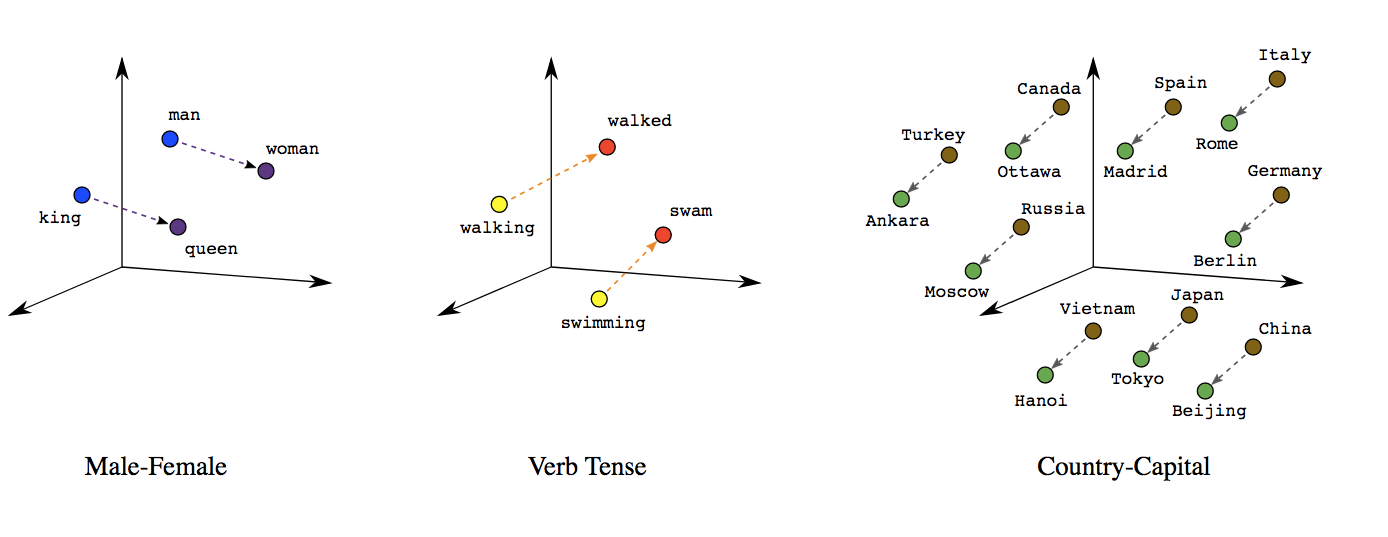
\includegraphics[width=0.95\linewidth]{img/lecture21/1_SYiW1MUZul1NvL1kc1RxwQ.png}
    \caption{Linear Relationships between Words.}
    \label{fig:word_embeddings}
\end{figure}

Encoder--Decoder architectures leverage these embeddings to create contextual representations of word sequences, enabling tasks such as machine translation. By embedding tokens in a continuous space, the Encoder can capture syntactic and semantic relationships in the input sequence, while the Decoder uses these learned representations to generate coherent and meaningful outputs. Unlike autoencoders, Encoder--Decoder models focus on transforming input sequences into context-rich outputs, making them essential for sequence-to-sequence applications.

\subsection{Word2Vec}

A widely used approach for learning word embeddings from large text corpora is the Word2Vec framework \cite{2,3}. Word2Vec learns vector representations by exploiting the idea that words appearing in similar contexts tend to have similar meanings, a concept rooted in the distributional hypothesis \cite{4}. Unlike traditional bag-of-words (BoW) representations, which encode word counts in sparse vectors without preserving semantic similarity, Word2Vec learns dense distributed representations in which similar words occupy nearby locations in embedding space. Instead of manually designing features, the model learns embeddings by solving a prediction task based on word co-occurrence. Two main training objectives are commonly used \cite{2}: the \textbf{Skip-Gram} model and the \textbf{Continuous Bag-of-Words (CBOW)} model.

For completeness, consider first the simplified \emph{one-word context} setting, where a single input word is mapped from a high-dimensional one-hot vector \(X \in \mathbb{R}^P\) to a lower-dimensional embedding \(Z \in \mathbb{R}^K\) with \(K < P\). This simplified formulation illustrates the basic mechanism by which embeddings are learned, but it is rarely used in practice because meaningful context typically depends on multiple surrounding words. 

Word2Vec models typically learn embeddings using one of two architectures.

\subsubsection*{Skip-Gram Model}

The \textbf{Skip-Gram} model learns embeddings by predicting surrounding context words given a target word \cite{2}. For a word sequence \(\{w_t\}_{t=1}^T\) and a context window of size \(k\), the Skip-Gram objective maximizes the probability of observing neighboring words \(w_{t-k}, \ldots, w_{t+k}\) (excluding the center word) given the target word \(w_t\):
\[
\sum_{t=1}^{T} \sum_{\substack{-k \le j \le k \\ j \neq 0}} 
\log P(w_{t+j}\mid w_t).
\]
The conditional probability is computed using a softmax over the dot product of learned word embeddings. Intuitively, the model adjusts embeddings so that words appearing in similar contexts obtain similar vector representations.

\subsubsection*{Continuous Bag-of-Words (CBOW)}

The \textbf{Continuous Bag-of-Words (CBOW)} model reverses the Skip-Gram prediction task \cite{2}. Instead of predicting surrounding words from a target word, CBOW predicts the target word from its surrounding context. The embeddings of the context words within a window are summed or averaged to form a single representation, which is then used to predict the center word:
\[
\sum_{t=1}^{T} \log P(w_t \mid w_{t-k}, \ldots, w_{t+k}).
\]
This objective encourages the model to learn embeddings that capture shared semantic and syntactic properties across context words.

\begin{figure}[H]
    \centering
    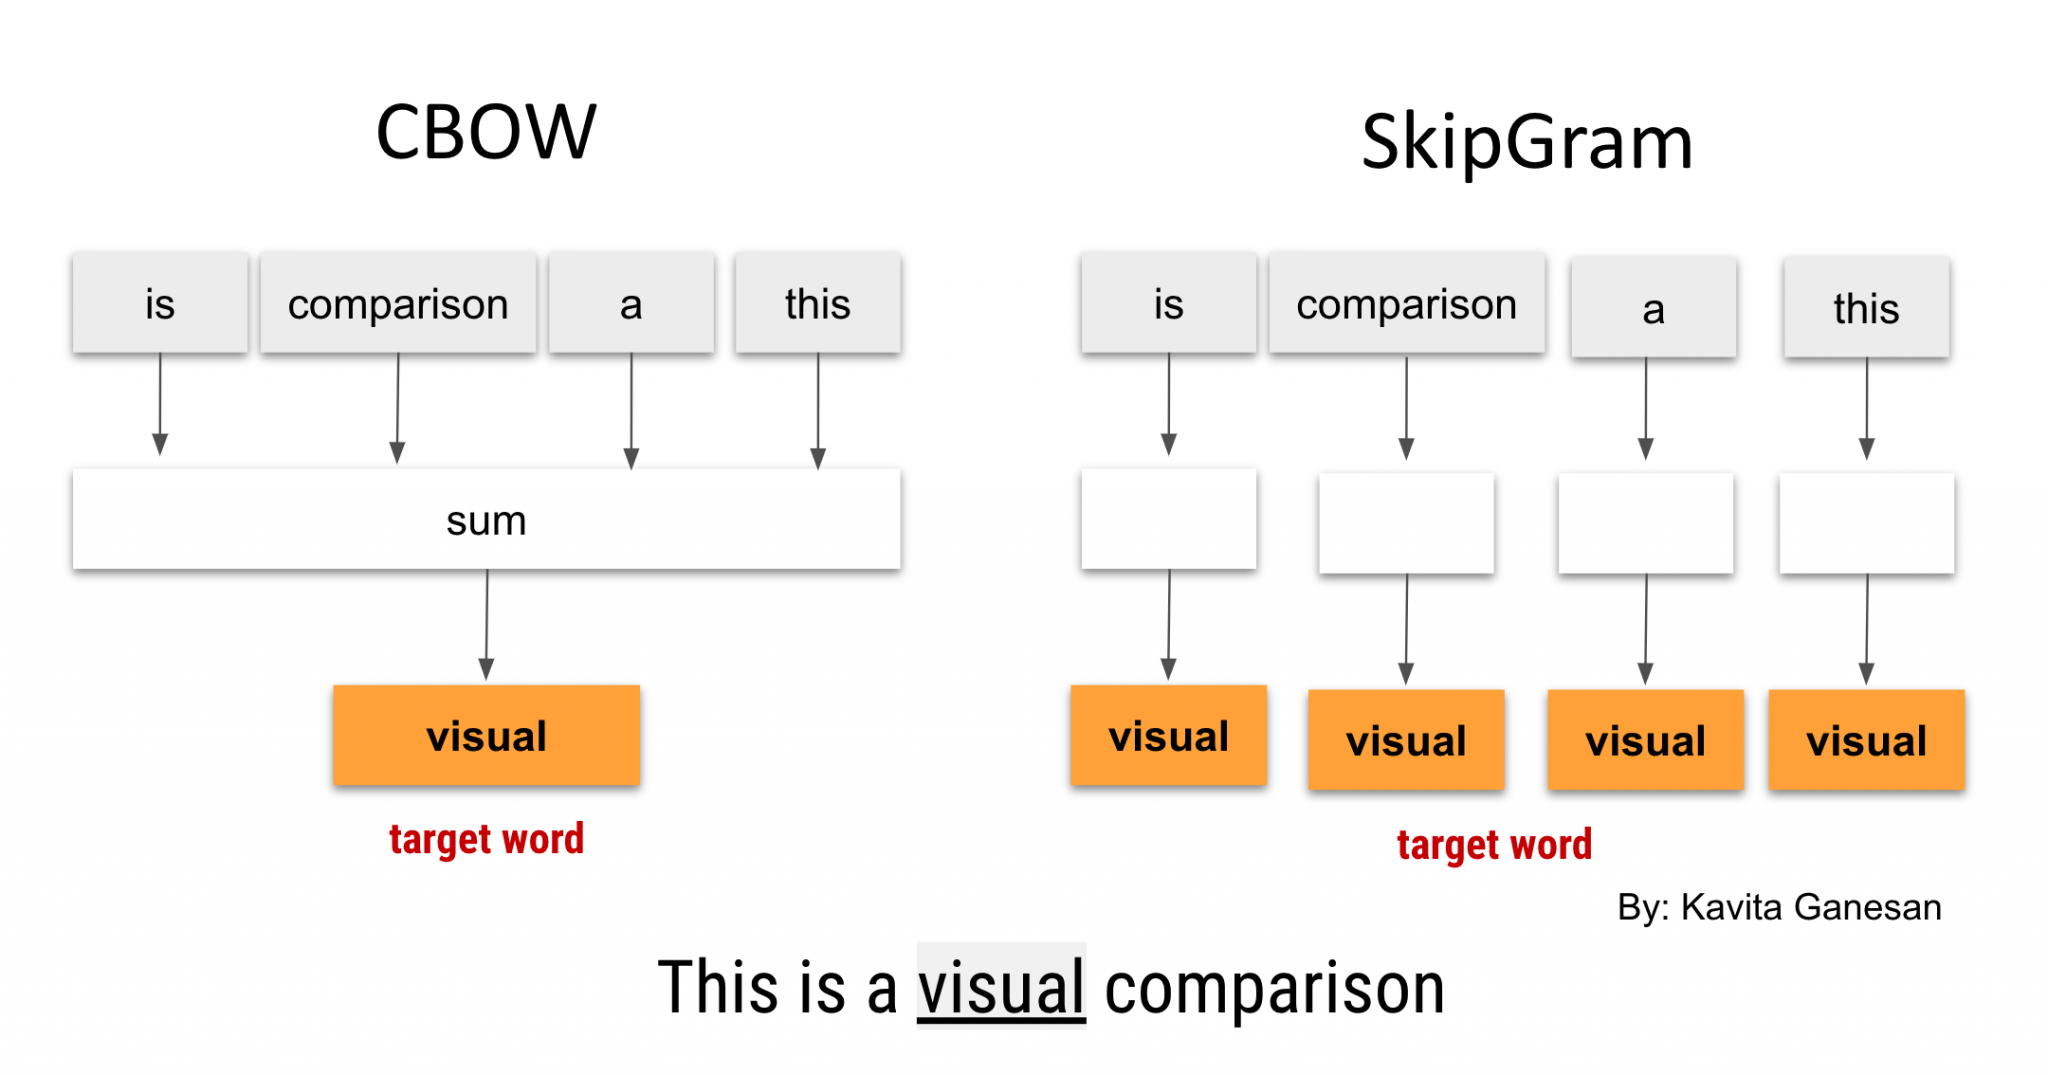
\includegraphics[width=0.74\linewidth]{img/lecture21/skipgram-vs-cbow-continuous-bag-of-words-word2vec-word-representation-2048x1075.png}
    \caption{Difference between Skip-Gram and CBOW training architectures.}
    \label{fig:skipgram_cbow}
\end{figure}

Both Skip-Gram and CBOW produce embeddings that capture semantic relationships and serve as foundational representations for many modern NLP architectures. These learned embeddings form the foundation for Encoder--Decoder architectures, enabling models to represent words in a continuous vector space and generate contextually meaningful sequences for applications such as machine translation and text summarization. 

\subsection{Sequence-to-Sequence (Seq2Seq) Model}

The \textbf{Sequence-to-Sequence (Seq2Seq)} model is a practical implementation of the Encoder--Decoder framework designed to handle variable-length input and output sequences, such as in machine translation \cite{6}. The \textbf{Encoder} processes an input sentence word by word and produces a sequence of hidden states, with the final hidden state summarizing the entire input sequence into a context vector.

\begin{figure}[H]
    \centering
    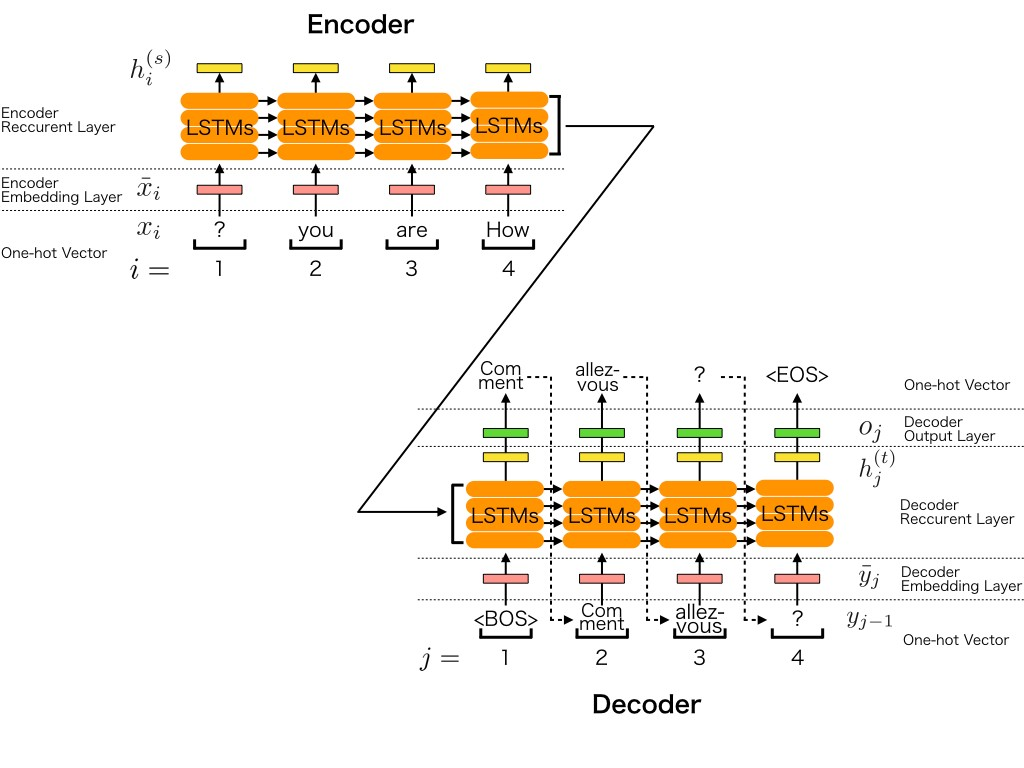
\includegraphics[width=0.8\linewidth]{img/lecture21/ezgif-5-d49a166959.jpg}
    \caption{LSTM-based Seq2Seq Encoder--Decoder Architecture}
    \label{fig:seq2seq_model}
\end{figure}

As illustrated in Figure~\ref{fig:seq2seq_model}, let \( x_i \) denote the input token at position \( i \), and let \( h_i \) denote the corresponding encoder hidden state. When the Encoder is implemented using Long Short-Term Memory (LSTM) units, the hidden state evolves as
\[
h_i = \text{LSTM}(x_i, h_{i-1}),
\]
where \( h_{i-1} \) is the previous hidden state. After the full input sequence has been processed, the final hidden state \( h_T \) becomes the context vector
\[
c = h_T,
\]
which summarizes the entire input sentence.

The \textbf{Decoder} generates the output sequence autoregressively, producing one token at a time. At decoding step \( j \), the Decoder uses the previously generated token \( y_{j-1} \), the previous hidden state \( s_{j-1} \), and the context vector \( c \) to update its hidden state:
\[
s_j = \text{LSTM}(y_{j-1}, s_{j-1}, c).
\]
The probability distribution over the next output token is then obtained by applying a softmax layer to \( s_j \). This process repeats until an end-of-sequence token is produced, allowing the model to generate output sequences of arbitrary length.

Seq2Seq models form the foundation of many modern sequence generation systems and paved the way for attention-based and Transformer architectures introduced later.

\subsection{Dot-Product Attention}

Although the Seq2Seq model performs well on short sequences, it struggles with longer inputs because the entire sentence must be compressed into a single fixed-size context vector, creating an information bottleneck \cite{7,8}. This bottleneck limits the model’s ability to retain detailed information. To address this limitation, \textbf{Dot-Product Attention} allows the Decoder to dynamically focus on different parts of the input sequence at each decoding step.

Instead of using a single context vector for all output steps, attention computes a \emph{new context vector} for every decoder step. At decoding step \( j \), the model measures how well the decoder hidden state \( s_j \) aligns with each encoder hidden state \( h_i \). This alignment score is computed using the dot product:
\[
e_{j,i} = s_j^{\top} h_i.
\]

These alignment scores are converted into attention weights using a softmax function:
\[
\alpha_{j,i} = 
\frac{\exp(e_{j,i})}
{\sum_{k=1}^{T} \exp(e_{j,k})}.
\]
The attention weight \( \alpha_{j,i} \) represents how much importance the Decoder assigns to encoder state \( h_i \) when generating the \( j \)-th output token.

The step-specific context vector is then computed as a weighted sum of the encoder hidden states:
\[
c_j = \sum_{i=1}^{T} \alpha_{j,i} h_i.
\]

This dynamically computed context vector \( c_j \) replaces the single fixed context vector used in basic Seq2Seq models. The Decoder uses \( c_j \) together with its hidden state to generate the next output token. By recomputing the context at each step, attention enables the model to selectively focus on the most relevant parts of the input sequence, significantly improving performance on long sequences.

Dot-product attention forms the basis for modern attention-based models and serves as the foundation for Transformer architectures introduced later \cite{8,11}.

\section{Attention-Based Encoder--Decoder Models}

While dot-product attention improves the basic Seq2Seq framework by allowing the decoder to focus on different encoder states at each output step, more structured attention mechanisms can further improve alignment quality and translation performance. In particular, Luong et al.\ proposed two broad classes of attention-based models: \emph{global attention}, which attends to all encoder hidden states, and \emph{local attention}, which restricts attention to a smaller window of source positions \cite{8}. These two variants differ in how the context vector is computed and in the trade-off they make between computational cost and alignment flexibility.

At decoder step \(t\), let the decoder hidden state be \(\mathbf{s}_t\), and let the encoder produce source-side hidden states \(\mathbf{h}_1, \mathbf{h}_2, \dots, \mathbf{h}_T\). In both global and local attention, the goal is to construct a context vector \(\mathbf{c}_t\) that summarizes the source information most relevant for predicting the current output token. This context vector is then combined with the decoder hidden state to form an attentional hidden representation:
\[
\tilde{\mathbf{s}}_t = \tanh\!\left(\mathbf{W}_c[\mathbf{c}_t;\mathbf{s}_t]\right),
\]
which is then used to produce the output distribution:
\[
P(y_t \mid y_{<t}, x) = \text{softmax}(\mathbf{W}_s \tilde{\mathbf{s}}_t).
\]

\subsection{Global Attention}

In the global attention model, the decoder considers \emph{all} encoder hidden states when forming the context vector \cite{8}. At decoding step \(t\), an alignment score is computed between the current decoder hidden state \(\mathbf{s}_t\) and each encoder hidden state \(\mathbf{h}_i\). In the simplest dot-product form, the score is
\[
e_{t,i} = \mathbf{s}_t^\top \mathbf{h}_i.
\]
These scores are normalized with a softmax to form attention weights:
\[
\alpha_{t,i} = \frac{\exp(e_{t,i})}{\sum_{k=1}^{T}\exp(e_{t,k})}.
\]
The context vector is then computed as a weighted sum of all encoder hidden states:
\[
\mathbf{c}_t = \sum_{i=1}^{T} \alpha_{t,i}\mathbf{h}_i.
\]

The key advantage of global attention is that it allows the decoder to examine the entire source sequence at every output step. This can yield strong alignment quality because the model is free to attend to any input position when generating the next token. However, this flexibility also comes with higher computational cost, especially for long input sequences, since attention weights must be computed over all encoder states at every decoding step.

\begin{figure}[H]
    \centering
    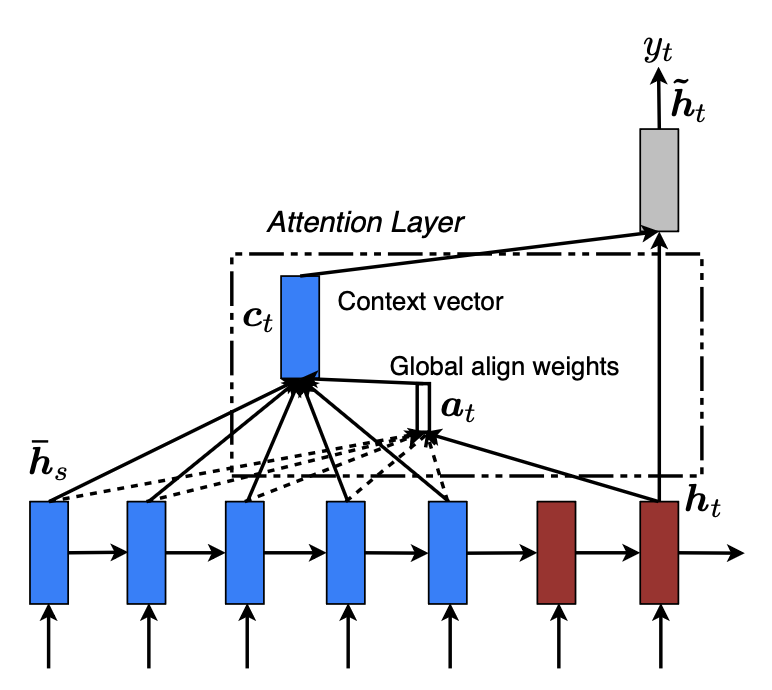
\includegraphics[width=0.72\linewidth]{img/lecture20/global_attention.png}
    \caption{Global attention model. At each decoder step, the model computes attention weights over all encoder hidden states and forms the context vector as their weighted average.}
    \label{fig:global_attention}
\end{figure}

\subsection{Local Attention}

Local attention reduces the computational burden of global attention by restricting the decoder to attend only to a small subset of encoder states \cite{8}. Instead of computing attention over the full source sequence, the model first predicts an aligned source position \(p_t\) for the current decoding step and then attends only to encoder states within a window centered at that position.

If the attention window has radius \(D\), the context vector is computed over the limited range
\[
i \in [p_t - D,\; p_t + D].
\]
Thus, the local context vector takes the form
\[
\mathbf{c}_t = \sum_{i=p_t-D}^{p_t+D} \alpha_{t,i}\mathbf{h}_i,
\]
where the attention weights are computed only within this window.

This restriction makes local attention more efficient than global attention, since the model no longer needs to compare the decoder state with every encoder state. At the same time, it preserves differentiability and usually retains strong alignment performance. In practice, local attention often provides a useful compromise: it is cheaper than global attention while still allowing the model to focus on the most relevant part of the source sequence. Luong et al.\ report that local attention can achieve performance comparable to, and in some cases better than, the global approach \cite{8}.

\begin{figure}[H]
    \centering
    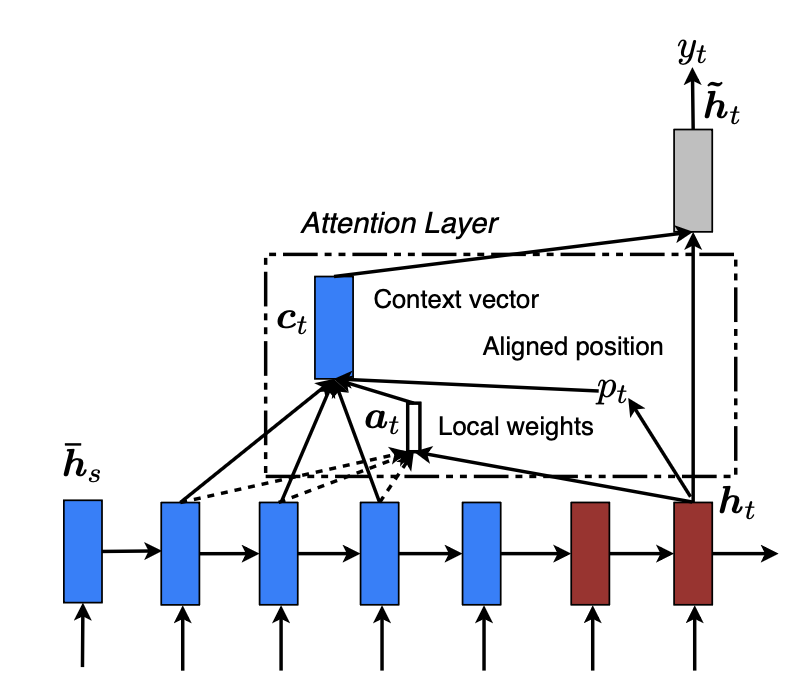
\includegraphics[width=0.72\linewidth]{img/lecture20/local_attention.png}
    \caption{Local attention model. At each decoder step, the model predicts an aligned source position and computes attention only within a window around that position.}
    \label{fig:local_attention}
\end{figure}

\subsection{Discussion}

Both global and local attention address the main limitation of the basic Seq2Seq model, namely the fixed-context bottleneck. Instead of relying on a single encoder summary vector for the entire output sequence, the decoder computes a new context vector at each step. Global attention provides maximum flexibility by considering all source positions, whereas local attention improves efficiency by narrowing the search to a neighborhood around a predicted alignment point. These ideas laid important groundwork for later attention-based models and helped motivate the transition from recurrent Seq2Seq architectures toward fully attention-based Transformer models \cite{8,11}.

% \section{Vision Transformer (ViT)}

% The \textbf{Vision Transformer (ViT)} adapts the Transformer architecture to image data by treating an image as a sequence of patches, analogous to treating a sentence as a sequence of tokens in NLP. Instead of using convolutional layers, ViT relies entirely on the self-attention mechanism introduced earlier. Each image patch is embedded into a vector representation, combined with positional information, and processed by a Transformer encoder.

% \subsection{Patchify Step in ViT}

% The first stage of ViT converts the image into a sequence of patch embeddings. 
% Given an input image 
% \[
% x \in \mathbb{R}^{H \times W \times C},
% \]
% where \(H\) and \(W\) denote the image height and width and \(C\) is the number of channels (e.g., \(C=3\) for RGB), the image is divided into non-overlapping square patches of size \(P \times P\).

% \begin{figure}[H]
%     \centering
%     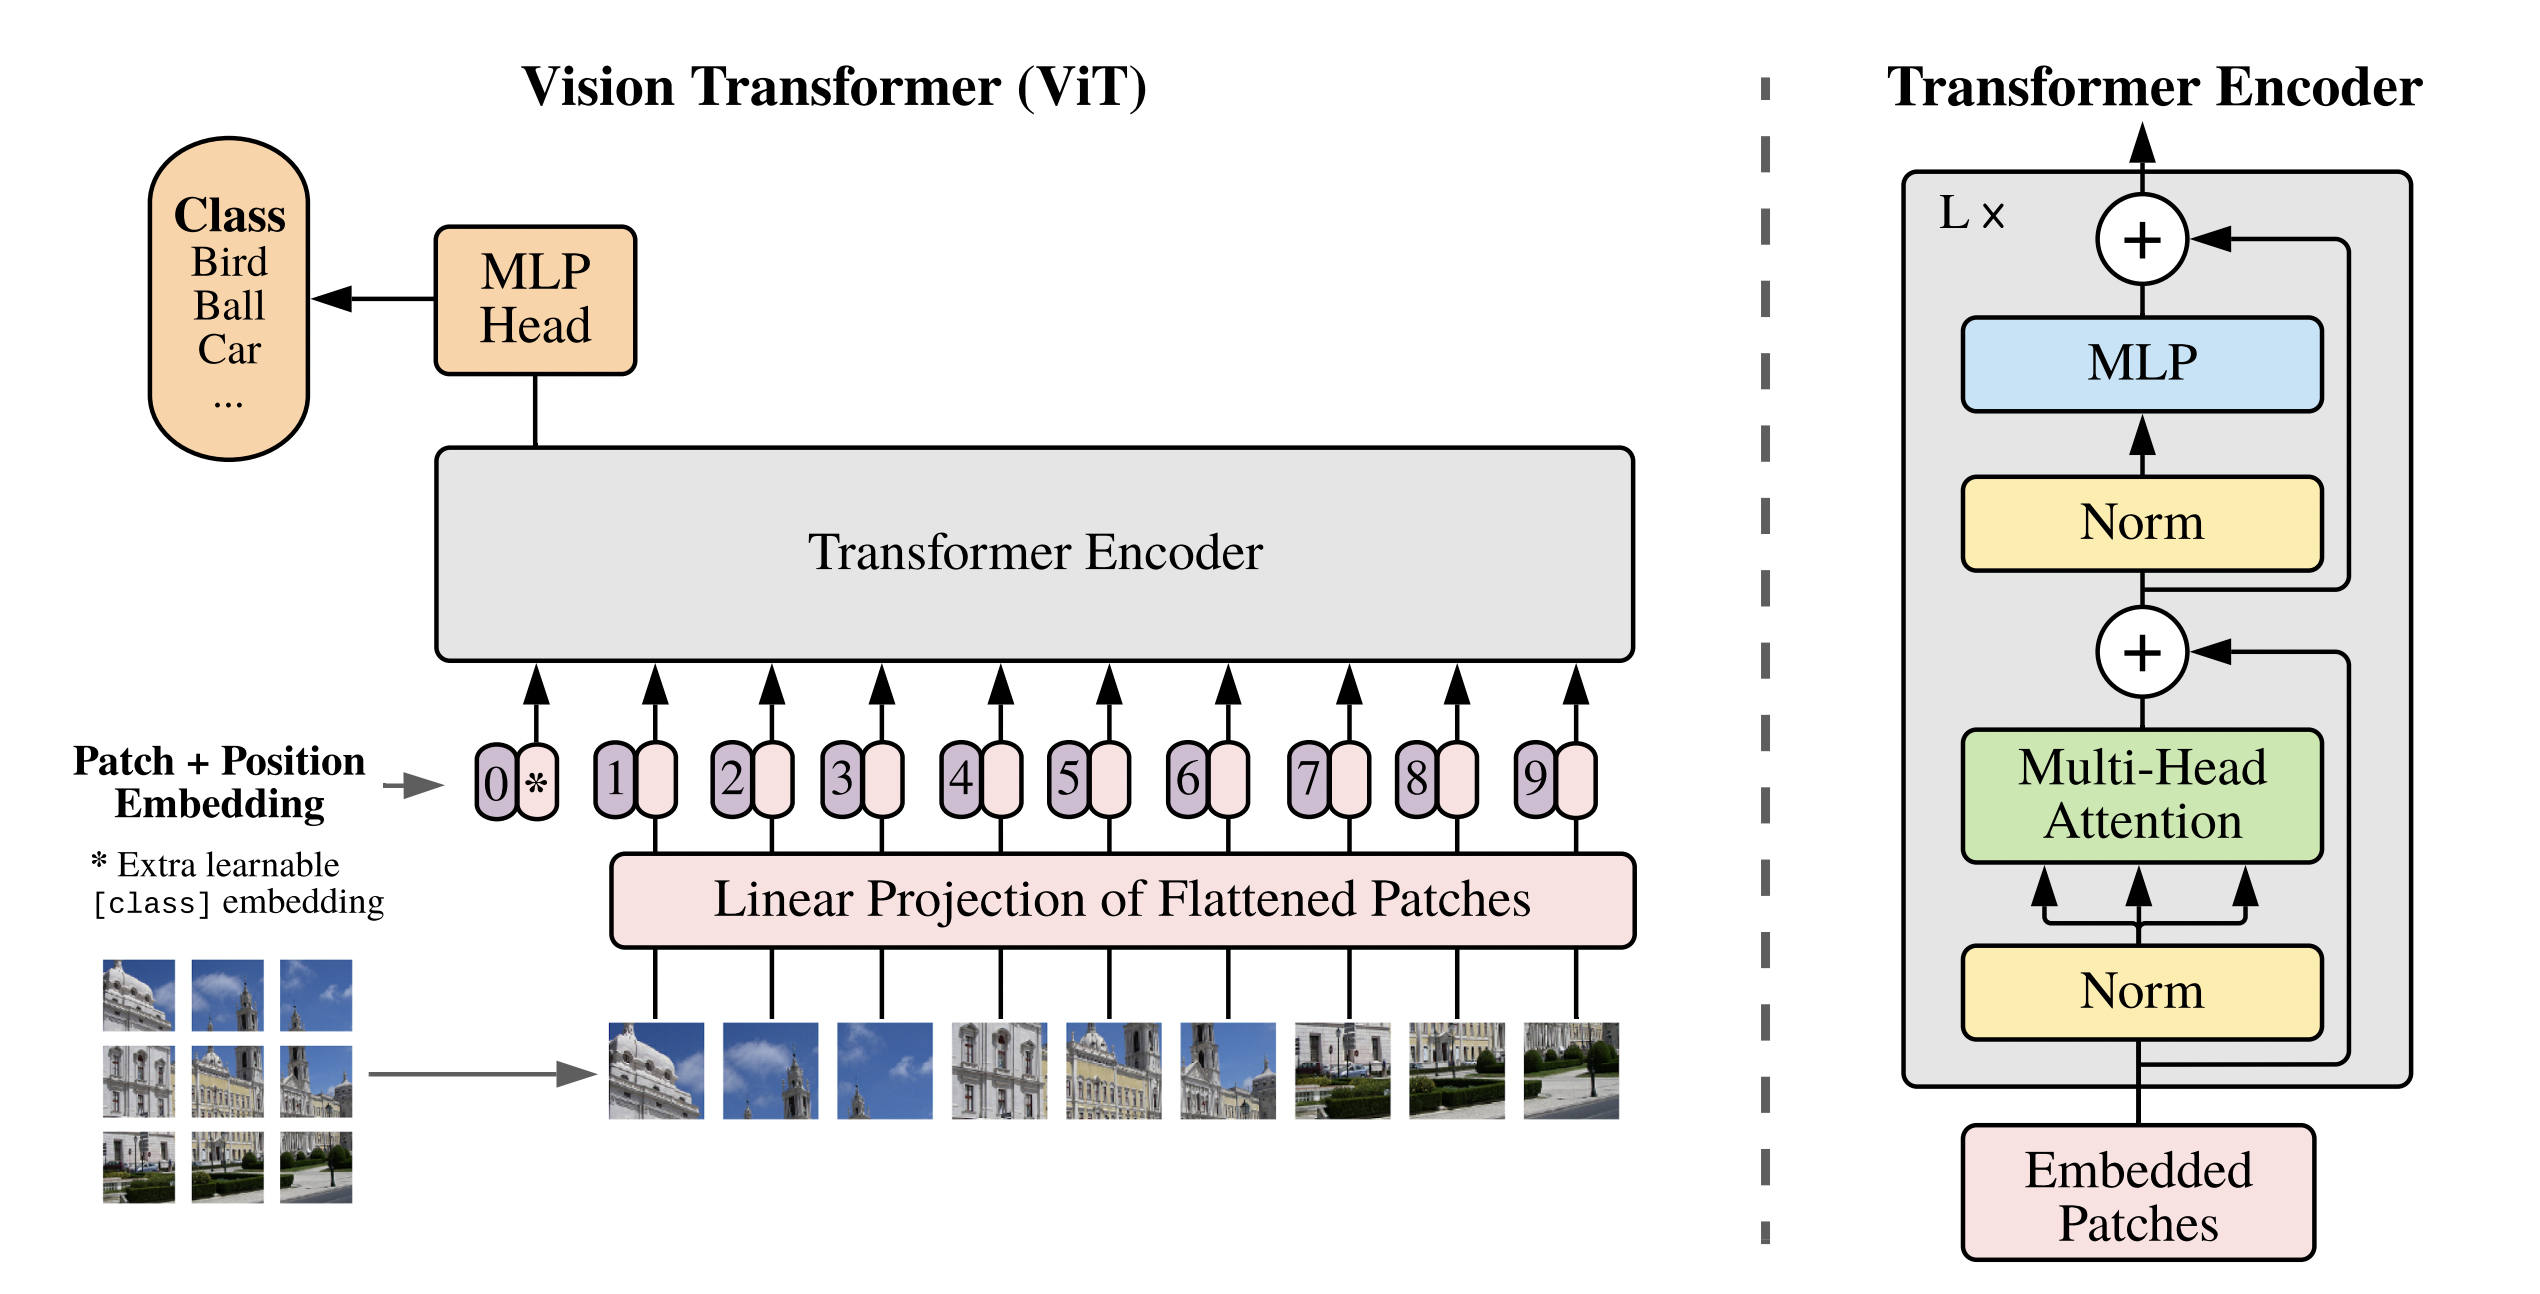
\includegraphics[width=1\linewidth]{img/lecture21/截圖 2024-11-10 下午5.15.24.png}
%     \caption{Vision Transformer (ViT) Architecture}
%     \label{fig:vit_architecture}
% \end{figure}

% The total number of patches produced is
% \[
% N = \frac{H \times W}{P^2}.
% \]
% Each patch is flattened into a vector of dimension \(P^2 C\), transforming the 2D image into a sequence of vectors. These vectors are then projected into a \(D\)-dimensional embedding space using a learnable linear transformation:
% \[
% z_p = x_p E,
% \]
% where \(x_p\) denotes a flattened patch and 
% \[
% E \in \mathbb{R}^{(P^2 C)\times D}
% \]
% is a learnable embedding matrix. This projection produces a sequence of patch embeddings that serve as input tokens to the Transformer encoder.

% Because flattening removes spatial ordering, ViT adds \textbf{positional embeddings} to each patch embedding. These learnable positional vectors encode where each patch originated in the image, allowing the Transformer to retain spatial structure.

% A special learnable \textbf{classification token} (denoted \texttt{[CLS]}) is then prepended to the sequence of patch embeddings. As the sequence passes through the Transformer encoder, this token aggregates information from all patches and is ultimately used for image classification.

% The resulting token sequence, consisting of the classification token and the patch embeddings, is processed by the Transformer encoder using multi-head self-attention. This design enables the model to capture global relationships between image regions, allowing it to reason about the entire image rather than relying on local convolutional filters.

% \subsection{Layer Normalization}

% Transformer models rely heavily on \textbf{Layer Normalization} to stabilize training. 
% While convolutional networks often use Batch Normalization, this technique is not well suited for sequence models because it depends on batch statistics and assumes consistent batch sizes. In sequence modeling and NLP tasks, batch sizes may vary and sequences can have different lengths, making Batch Normalization less reliable.

% Unlike Batch Normalization, which computes statistics across the batch dimension, Layer Normalization normalizes \emph{within each token}. This means the normalization is computed across the feature dimension of a single token, making the operation independent of batch size and sequence length. As a result, Layer Normalization works consistently during both training and inference.

% Given an input feature vector \( x \), Layer Normalization is defined as:
% \[
% y = \frac{x - \mathbb{E}[x]}{\sqrt{\text{Var}[x] + \epsilon}} \cdot \gamma + \beta
% \]
% where \( \mathbb{E}[x] \) and \( \text{Var}[x] \) are the mean and variance computed across the features of the token. The learnable parameters \( \gamma \) and \( \beta \) allow the model to scale and shift the normalized output. This transformation standardizes the representation of each token and helps maintain stable gradients throughout deep transformer networks.

% Because Layer Normalization does not rely on running statistics, it avoids discrepancies between training and inference and reduces memory overhead. These properties make it particularly well suited for Transformer architectures, where normalization is applied repeatedly within attention and feed-forward blocks.

% \begin{figure}[H]
%     \centering
%     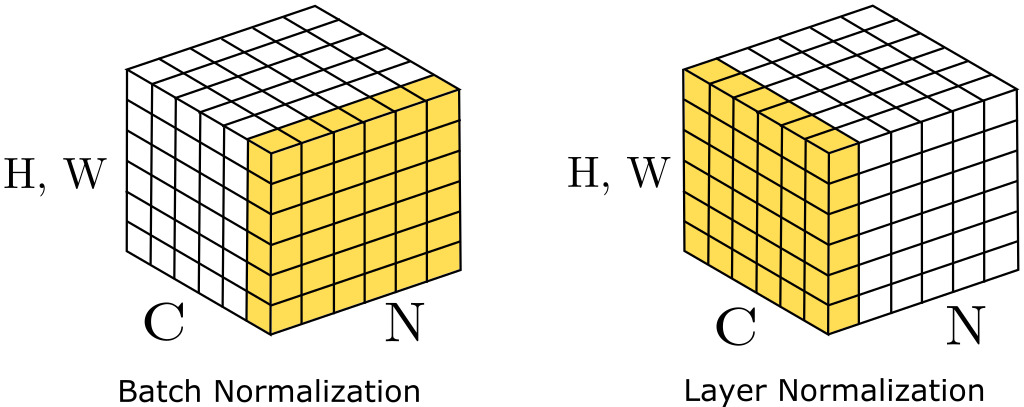
\includegraphics[width=0.6\linewidth]{img/lecture21/e068e06a.png}
%     \caption{Comparison of Batch Normalization and Layer Normalization. Batch normalization computes statistics across the batch dimension, whereas layer normalization computes statistics across the feature dimension of each token independently.}
%     \label{fig:layer_norm}
% \end{figure}

% \subsection{Attention Mechanism}

% Attention is the core operation that enables transformer models to dynamically focus on the most relevant parts of an input sequence. This capability is especially important in sequence modeling tasks, where the importance of tokens varies depending on context.

% Attention is computed using three matrices derived from the input sequence: the \textbf{query} \(Q\), the \textbf{key} \(K\), and the \textbf{value} \(V\). The similarity between tokens is measured by taking the dot product between queries and keys to produce attention scores. These scores are scaled by \( \sqrt{d_k} \), where \( d_k \) is the dimensionality of the key vectors, to stabilize gradients during training. The scaled dot-product attention is defined as:
% \[
% \text{Attention}(Q, K, V) = \text{softmax}\!\left(\frac{QK^{\top}}{\sqrt{d_k}}\right)V
% \]
% The softmax operation converts the scores into attention weights, which determine how strongly each token influences the final representation. Applying these weights to the value vectors produces a context-aware output that captures both local and long-range dependencies within the sequence.

% Transformers further extend this idea through \textbf{multi-head attention}. Instead of computing a single attention distribution, the model uses multiple attention heads, each learning different relationships within the data. The outputs of all heads are concatenated and projected using a learnable matrix \(W_O\):
% \[
% \text{MultiHead}(Q, K, V) = \text{Concat}(\text{head}_1,\dots,\text{head}_h) W_O
% \]
% Each attention head operates on a different learned projection of the inputs:
% \[
% \text{head}_i = \text{Attention}(QW_i^Q,\; KW_i^K,\; VW_i^V)
% \]
% This multi-head design allows the transformer to simultaneously capture multiple types of relationships, such as syntactic structure and long-range semantic dependencies.

\begin{figure}[H]
    \centering
    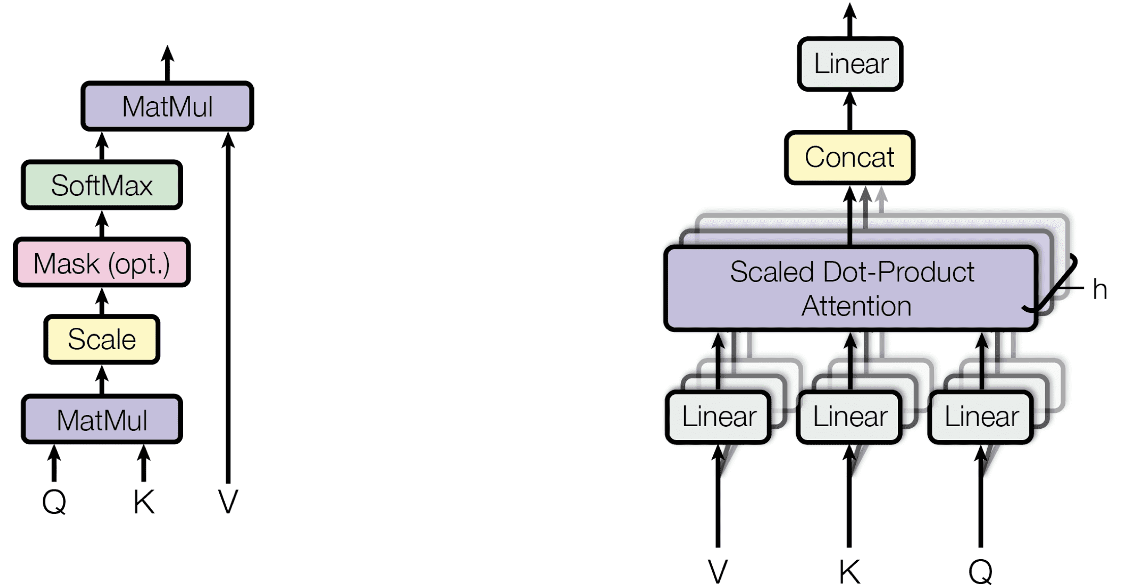
\includegraphics[width=0.7\linewidth]{img/lecture21/圖片 1.png}
    \caption{Scaled dot-product attention (left) and multi-head attention (right) used in transformer architectures.}
    \label{fig:attention}
\end{figure}

\section{Q\&A Section}

\begin{enumerate}

% ---------------- TCN ----------------

\item \textbf{Question:}
What makes a Temporal Convolutional Network (TCN) \emph{causal}, and how do dilated convolutions help it model long-range dependencies efficiently?

\textbf{Solution:}
A TCN is causal if the output at time $t$ depends only on inputs at times $\le t$, ensuring no information from the future is used. With kernel size $k$, a causal convolution computes:
\[
\mathbf{y}^{(t)} = f(\mathbf{x}^{(t)}, \mathbf{x}^{(t-1)}, \dots, \mathbf{x}^{(t-k+1)}).
\]
Dilated convolutions introduce a spacing factor $d$, expanding the receptive field:
\[
\mathbf{y}^{(t)} = f(\mathbf{x}^{(t)}, \mathbf{x}^{(t-d)}, \dots, \mathbf{x}^{(t-d(k-1))}).
\]
Using dilation factors such as $1,2,4,8,\dots$ across layers increases the receptive field exponentially while keeping the number of parameters per layer fixed.

\item \textbf{Question:}
For a TCN with kernel size $k=3$ and dilation factors $1,2,4$, what is the receptive field?

\textbf{Solution:}
\[
R = 1 + \sum_{\ell}(k-1)d_\ell
= 1 + 2(1+2+4)
= 15.
\]
Thus, the output at time $t$ depends on inputs from $t$ back to $t-14$.

% ---------------- Seq2Seq ----------------

\item \textbf{Question:}
What is the main limitation of the basic Seq2Seq model without attention?

\textbf{Solution:}
The encoder compresses the entire input sequence into a single fixed-size context vector $c = h_T$. For long sequences, this vector may not retain all relevant information, creating an information bottleneck that degrades performance.

\item \textbf{Question:}
How does dot-product attention address the Seq2Seq bottleneck?

\textbf{Solution:}
Instead of using one fixed context vector, attention computes a dynamic context vector at each decoding step:
\[
\alpha_{j,i} = \frac{\exp(s_j^\top h_i)}{\sum_k \exp(s_j^\top h_k)}, 
\qquad
c_j = \sum_i \alpha_{j,i} h_i.
\]
This allows the decoder to focus on different parts of the input for each output token.

% ---------------- Transformer ----------------

\item \textbf{Question:}
What is the formula for scaled dot-product attention, and why is scaling necessary?

\textbf{Solution:}
\[
\text{Attention}(Q,K,V)
= \text{softmax}\!\left(\frac{QK^\top}{\sqrt{d_k}}\right)V.
\]
The scaling by $\sqrt{d_k}$ prevents the dot products from growing too large when $d_k$ is large, which would otherwise push the softmax into regions with very small gradients.

\item \textbf{Question:}
Why does multi-head attention improve model capacity?

\textbf{Solution:}
Each attention head learns separate projections:
\[
\text{head}_i = \text{Attention}(QW_i^Q, KW_i^K, VW_i^V).
\]
Multiple heads allow the model to attend to different relationships (e.g., syntactic vs. semantic structure) simultaneously.

% ---------------- Layer Norm ----------------

\item \textbf{Question:}
Why is layer normalization preferred over batch normalization in transformers?

\textbf{Solution:}
Layer normalization computes statistics across features within each token:
\[
y = \frac{x - \mathbb{E}[x]}{\sqrt{\mathrm{Var}[x]+\epsilon}}\gamma + \beta.
\]
It does not depend on batch statistics, making it stable for varying batch sizes and sequence lengths, and consistent during inference.

% ---------------- Word2Vec ----------------

\item \textbf{Question:}
What is the difference between Skip-Gram and CBOW in Word2Vec?

\textbf{Solution:}
Skip-Gram predicts surrounding context words given a target word:
\[
\sum_{t}\sum_{j\neq0} \log P(w_{t+j}\mid w_t).
\]
CBOW predicts the target word from its surrounding context:
\[
\sum_t \log P(w_t\mid w_{t-k},\dots,w_{t+k}).
\]
Skip-Gram works well for rare words; CBOW is computationally more efficient.

\end{enumerate}


\section{References}

\beginrefs

\bibentry{1} Y. Bengio, R. Ducharme, P. Vincent, and C. Janvin. 
A neural probabilistic language model. 
Journal of Machine Learning Research, 3:1137--1155, 2003.

\bibentry{2} T. Mikolov, K. Chen, G. Corrado, and J. Dean.
Efficient estimation of word representations in vector space.
arXiv preprint arXiv:1301.3781, 2013.

\bibentry{3} T. Mikolov, I. Sutskever, K. Chen, G. Corrado, and J. Dean.
Distributed representations of words and phrases and their compositionality.
Advances in Neural Information Processing Systems (NeurIPS), 2013.

\bibentry{4} Z. S. Harris.
Distributional structure.
Word, 10(2--3):146--162, 1954.

\bibentry{5} K. Cho, B. van Merri\"enboer, D. Bahdanau, and Y. Bengio.
On the properties of neural machine translation: Encoder--decoder approaches.
SSST-8, Eighth Workshop on Syntax, Semantics and Structure in Statistical Translation, 2014.

\bibentry{6} I. Sutskever, O. Vinyals, and Q. V. Le.
Sequence to sequence learning with neural networks.
Advances in Neural Information Processing Systems (NeurIPS), 2014.

\bibentry{7} D. Bahdanau, K. Cho, and Y. Bengio.
Neural machine translation by jointly learning to align and translate.
International Conference on Learning Representations (ICLR), 2015.

\bibentry{8} M.-T. Luong, H. Pham, and C. D. Manning.
Effective approaches to attention-based neural machine translation.
Proceedings of EMNLP, 2015.

\bibentry{9} T. Salimans and D. P. Kingma.
Weight normalization: A simple reparameterization to accelerate training of deep neural networks.
Advances in Neural Information Processing Systems (NeurIPS), 2016.

\bibentry{10} S. Bai, J. Z. Kolter, and V. Koltun.
An empirical evaluation of generic convolutional and recurrent networks for sequence modeling.
arXiv preprint arXiv:1803.01271, 2018.

\bibentry{11} A. Vaswani, N. Shazeer, N. Parmar, J. Uszkoreit, L. Jones, A. N. Gomez, L. Kaiser, and I. Polosukhin.
Attention is all you need.
Advances in Neural Information Processing Systems (NeurIPS), 2017.

\endrefs


\end{document}
